\chapter{Simulace ve virtuálním prostředí}

Simulátory umožňují letovému kódu PX4 ovládat počítačově modelované vozidlo v simulovaném \uv{světě}. S tímto vozidlem můžete komunikovat stejně jako se skutečným vozidlem pomocí QGroundControl, offboard API nebo rádiového ovladače/gamepadu. 

PX4 podporuje jak simulaci Software In the Loop (SITL), kde program letového ovladače běží na počítači, nebo simulaci Hardware In the Loop (HITL), kde simulační firmware běží na skutečném letovém ovladači. \cite{SIM}

Všechny simulátory můžou komunikovat s firmware PX4 pomocí \textit{Simulator MAVLink API}, které definuje sadu zpráv MAVLink. Na obrázku \ref{fig:SIM1} je zobrazen tok zpráv mezi \uv{simulovaným světem} a mezi firmware PX4. Další možnost komunikace mezi simulátorem a PX4 firmware využívá \textit{Micro-RTPS bridge}.

\begin{figure}[!ht]
  \begin{center}
    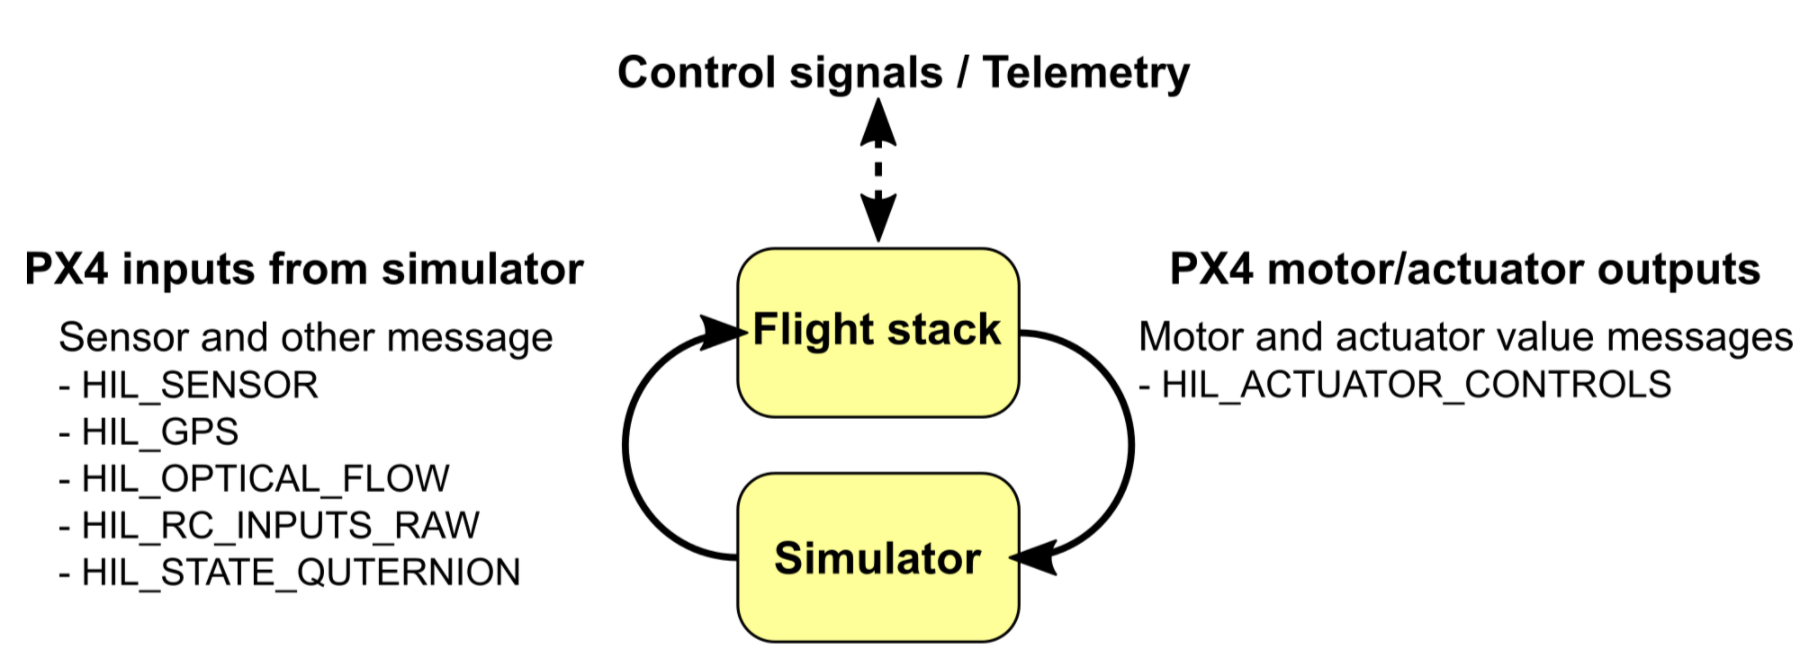
\includegraphics[scale=0.31]{obrazky/SIM1}
  \end{center}
  \caption[Tok zpráv mezi simulátorem a PX4]{Tok zpráv mezi simulátorem a PX4 \cite{SIM}.}
  \label{fig:SIM1}
\end{figure}

\section{SITL simulační prostředí}

\textit{Software In The Loop} simulace umožňuje rychlé a \uv{levné} ladění robotických misí, protože pro simulaci SITL se nevyužívá žádný specializovaný hardware, ale jenom počítač s nainstalovaným simulačním prostředím.

Obrázek \ref{fig:SIM2} zobrazuje typické prostředí simulace SITL v PX4 pro kterýkoliv z podporovaných simulátorů. Simulátor a PX4 firmawe můžou spolu komunikovat pomocí MAVLink \acs{API}. Pro přímou interakci s PX4 se využívá komunikace přes \textit{Micro-RTPS bridge}, kde se komunikují přímo uORB zprávy.

Různé části simulačního prostředí spolu komunikují pomocí \acs{UDP} (\acl{UDP}) a můžou být spuštěny na stejném počítači, nebo jiném počítači ve stejné síti. Pomocí sériové komunikace je možné připojit joystick, gamepad nebo RC soupravu pro ruční ovládání dronu přes QGroundControl.

\begin{figure}[!ht]
  \begin{center}
    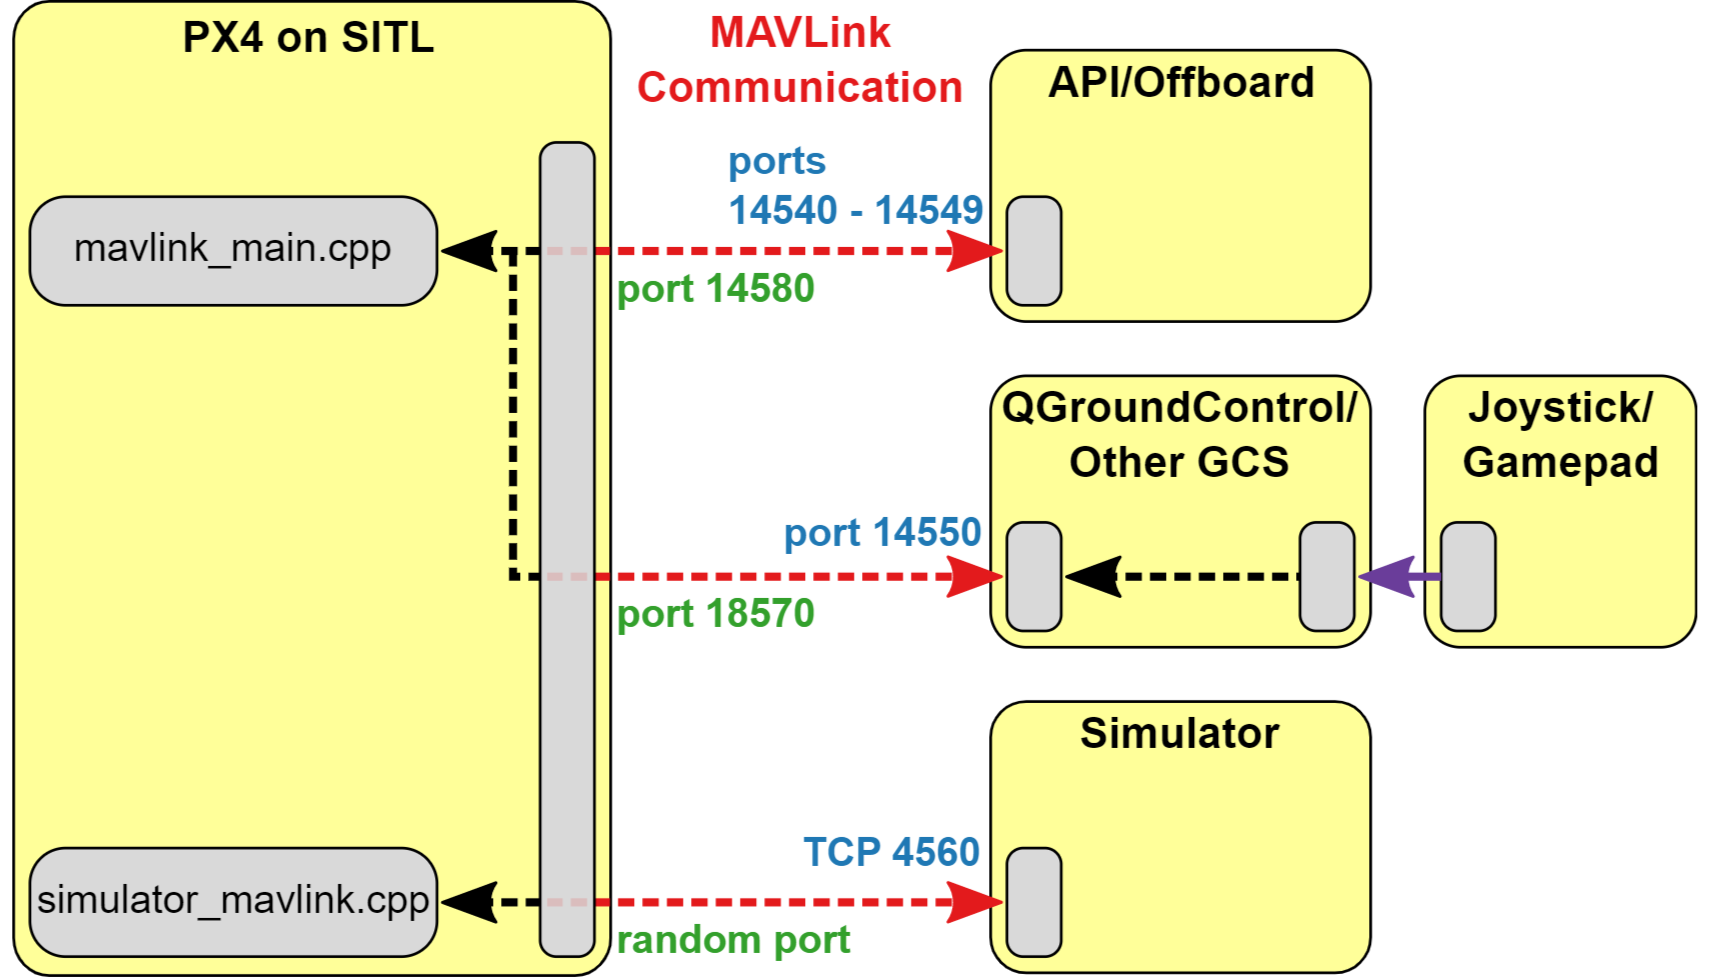
\includegraphics[scale=0.3]{obrazky/SIM2}
  \end{center}
  \caption[Diagram komunikace mezi PX4 a simulátorem]{Diagram komunikace mezi PX4 a simulátorem \cite{SIM}.}
  \label{fig:SIM2}
\end{figure}

\subsection{Seznam podporovaných simulátorů}

Následující simulátory jsou podporovány systémem PX4:

\begin{itemize}
    \item Gazebo
    \item FlightGear
    \item JSBSim
    \item jMAVSim
    \item AirSim
    \item Ignition Gazebo
\end{itemize}

\subsection{Gazebo}

Simulátor Gazebo je vysoce doporučen pro PX4 simulaci.

Gazebo je dobře navržený simulátor, umožňující rychlé testovávaní algoritmů, návrh robotů a trénování systémů s umělou inteligencí v realistických scénářích. Nabízí možnost přesně a efektivně simulovat populace robotů ve složitých vnitřních i venkovních prostředích. Gazebo se běžně používá pro práci s ROS (ROS 2). \cite{GAZ}

Podporovaná vozidla v simulátoru Gazebo jsou:

\begin{itemize}
    \item dron
    \item delta \acs{VTOL} (\acl{VTOL})
    \item letadlo
    \item rover
    \item ponorka
\end{itemize}

\subsection{Ignition Gazebo}

Vývojový tím simulátoru Gazebo se v budoucnu zaměří na vývoj simulátoru Ignition, takže Gazebo 11 je poslední verze známého simulátoru. Tyto simulátory jsou kompatibilní ve formátu popisu prostředí (\uv{světa}) a některých pluginů. \cite{IGN}

Z důvodu, že simulační firmware PX4 je v této době lépe propojený se simulátorem Gazebo, tak v této práci budeme pracovat s simulátorem Gazebo 11.

Jediné vozidlo, které je podporované v simulátoru Ignition je dron.

\section{Instalace virtuálního prostředí}

\subsection{Instalace a nastavení ROS 2}

\subsection{Instalace PX4}

\subsection{Instalace simulátoru Gazebo}

\section{ROS 2 misie}

\subsection{Offboard flight mode}
